\documentclass[a4paper,12pt]{article}

%% Language and font encodings
\usepackage[francais]{babel}
\usepackage[utf8x]{inputenc}
\usepackage[T1]{fontenc}

%% Sets page size and margins
\usepackage[a4paper,top=3cm,bottom=2cm,left=3cm,right=3cm,marginparwidth=1.75cm]{geometry}

%% Useful packages
\usepackage{amsmath}
\usepackage{graphicx}
\usepackage{hyperref}

\title{Compte rendu projet IGR203}
\author{Alexis Bauvin -- Clément Decoodt -- Ronan Desplanques -- Ming Yang}

\begin{document}
\maketitle

\tableofcontents

\section*{Introduction}

Le projet que nous avons choisi est le projet de la carte de restaurant interactive. En effet, ce projet laisse une
certaine marge de manœuvre dans le design à implémenter.

Ce projet consiste à réaliser une carte interactive pour un restaurant à destination des clients. La façon dont nous
avons imaginé ce projet comporte deux formes : une application sur tablette, distribuée par le serveur à un client à
table et une application sur téléphone pour un client hors du restaurant, désireux de commander à distance.

\newpage

\section{Le design}

\subsection{Les pistes explorées}

\subsubsection{Design adapté à une tablette}

La première piste de design est adaptée à un écran de tablette. Elle utilise la taille de ce support pour proposer
une interface originale et agréable en plus d'être fonctionnelle. Il est fait usage de métaphores qui rappellent
les cartes de restaurant traditionnelles et la partie de l'interface qui exprime l'état courant de la commande
a la forme d'une table de restaurant où les éléments choisis sont disposés.

\subsubsection{Design adapté à un téléphone}

Cette idée de design correspond à une implémentation sur téléphone. Sur un écran plutôt petit, elle privilégie la
simplicité et la clarté en utilisant une interface de listes. Les boutons sont grands et occupent tout l'écran,
il n'y a pas d'éléments de décoration.

\subsubsection{Design traditionnel}

Ce design est fondé sur l'idée d'émuler au maximum une carte de menu classique. La partie principale de l'interface
prend la forme d'un menu traditionnel, et ce n'est qu'en touchant un élément qu'on peut accéder à des informations
spécifiques et commander. Pour accentuer l'aspect <<~papier~>> de l'interface, on reprend des caractéristiques des
liseuses électroniques comme les animations de tournage de page et la teinte du fond d'écran.

\subsection{Le design choisi}

Le premier design proposé a été choisi pour l'interface principale du système. C'est celui qui permet d'apporter
le plus de valeur ajoutée par rapport au système classique, et les contraintes techniques de son implémentation
ne paraissent pas insurmontables. Les besoins de personnalisation et d'interactivité de l'interface sont bien remplis
par le design. Le design est intuitif et ne nécessite pas de phase d'apprentissage pour être fonctionnel~: le
principe de <<~recognition over recall~>> est respecté.

Les objectifs les moins bien remplis par ce design sont les exigences de portabilité~: pour être correctement utilisée,
l'interface doit être disposée sur un grand écran, autant en taille physique que en définition. Ce design n'est donc
efficace que sur une tablette au minimum, il n'est donc pas destiné pour être utilisé par les clients sur leur propre
téléphone.

Pour répondre à ce dernier point, une version alternative de l'interface, plus sobre et suivant le deuxième design,
sera développée.

\subsection{Évolution des besoins lors de la conception du design}

Il n'a pas été possible de concilier tous les différents besoins dans un design unique. La difficulté fut de proposer
un aspect et des fonctionnalités suffisamment attrayants pour justifier un passage à un système numérique au niveau
de la carte des menus pour les clients sur place, et qui pourrait en même temps être portés sur les machines
personnelles des clients qui commandent à distance.

La solution est de proposer deux clients différents, avec le gros du développement dédié à l'interface principale
pour tablette. Cela ne propage pas une redondance à tout le système puisque la partie logique et celle présentée
au personnel du restaurant reste unique.

\subsection{Fonctionnement du design}

Cette partie explique en détail l'interface principale retenue et son fonctionnement : interactions, concepts, ...

\subsubsection{L'écran d'introduction}

L'écran d'introduction est ce qui est présenté avant le début de l'interaction d'un utilisateur avec le système.
L'utilisateur est invité à choisir entre <<~sur place~>> et <<~à emporter~>> pour commencer sa commande. La langue par
défaut est le français, mais un bouton avec une apparence de drapeau est affiché dans un coin. Celui-ci permet de
changer la langue de l'interface.

\begin{center}
	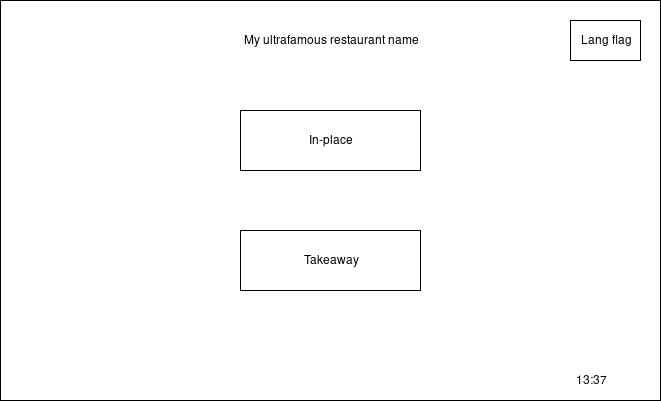
\includegraphics[width=\textwidth]{intro_screen.jpg}
\end{center}

Une disposition différente a également été envisagée :

\begin{center}
	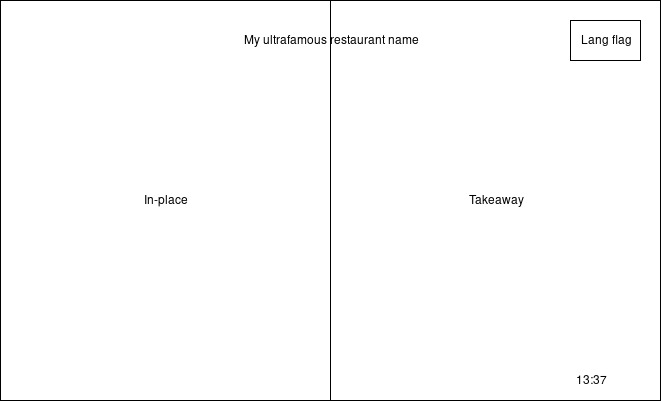
\includegraphics[width=\textwidth]{alt_intro_screen.jpg}
\end{center}

\subsubsection{L'écran principal après avoir choisi <<~sur place~>>}

Cette partie de l'interface repose sur deux <<~decks~>> : l'un en bas de l'écran et l'autre à droite. Celui de droite
permet de sélectionner le sous-menu correspondant à un type d'article, par exemple plats, desserts, boissons. Celui
du bas permet de sélectionner un article au sein d'une catégorie, par exemple coq au vin, croque-monsieur. Le bouton
drapeau reste présent sur cet écran comme sur tous les autres de l'interface.

\begin{center}
	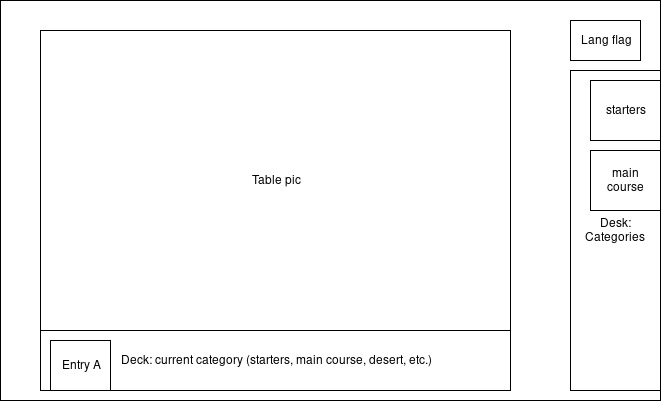
\includegraphics[width=\textwidth]{in_place_screen1.jpg}
\end{center}

Quand on clique sur un article, un écran modal s'ouvre et affiche des détails sur l'article et permet de préciser
quelques éléments (par exemple la cuisson pour une viande) avant de l'ajouter à la commande.

\begin{center}
	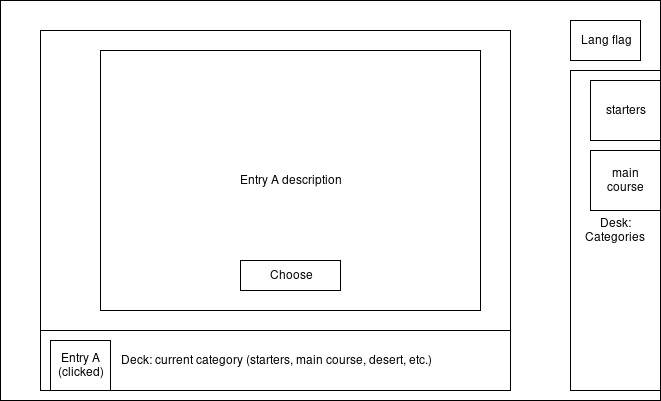
\includegraphics[width=\textwidth]{in_place_screen2.jpg}
\end{center}

La sélection se fait avec un concept de <<~deck de cartes~>> : chaque carte représente un élément, que l'on ajoute
en faisant glisser la carte. Pour sélectionner un plat dans le deck du bas, on <<~prend~>> la carte avec le doigt que
l'on <<~dépose~>> ensuite au centre de l'écran.

\begin{center}
	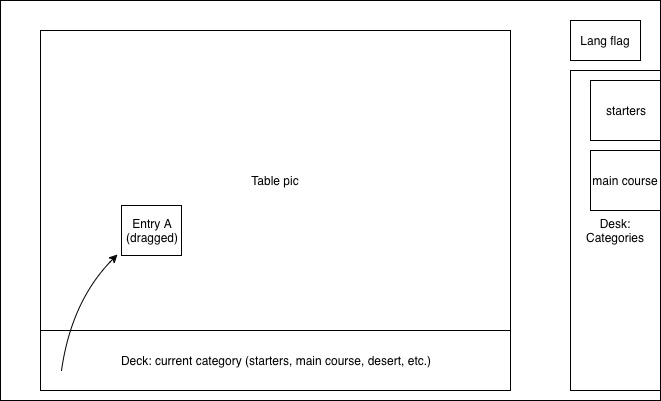
\includegraphics[width=\textwidth]{in_place_drag.jpg}
\end{center}

Le mécanisme est le même pour changer de catégorie du menu. L'on attrape une carte dans le deck de droite (par
exemple <<~entrées~>>) que l'on viens ensuite déposer sur le deck du bas, ce qui aura pour effet d'y distribuer
les cartes des nouveaux éléments.

La partie du centre de l'écran est l'image d'une table permettant de visualiser sa commande : au fur et à mesure que
l'on viens compléter sa commande, la table se garnit des éléments que l'on commande.

Le système de drag-and-drop permet d'ajouter un mécanisme de choix intuitif. Prenons l'exemple d'un steak : il est
important que le client puisse choisir la cuisson -- bien que <<~à point~>> devrait être bannie. Lorsqu'une carte
propose plusieurs choix comme ceci, des zones de surbrillance apparaissent au dessus de la table, correspondant
chacune à une option. Dans le cas de notre steak, trois zones seraient présentes : <<~saignant~>>, <<~moyen~>> et
<<~à point~>>. L'option retenue sera celle dans laquelle le client lâchera la carte.

\begin{center}
	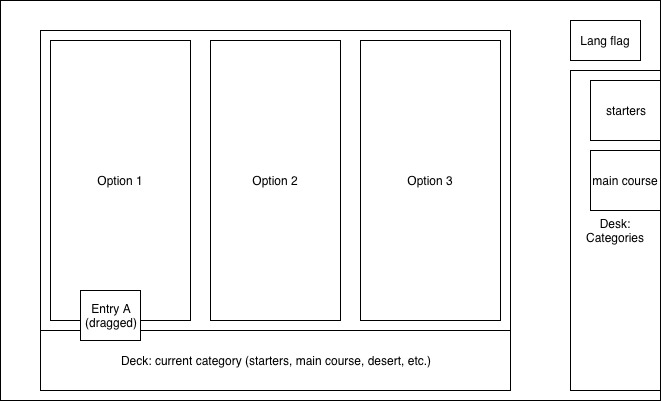
\includegraphics[width=\textwidth]{in_place_drag_options.jpg}
\end{center}

\subsubsection{L'écran après avoir choisi <<~à emporter~>>}

L'interface est plus sommaire et fonctionnelle sur cet écran~: les articles sont présentés dans une liste hiérarchisée
en sous-catégories. Le système d'écran modal du mode <<~sur place~>> est aussi présent.

\begin{center}
	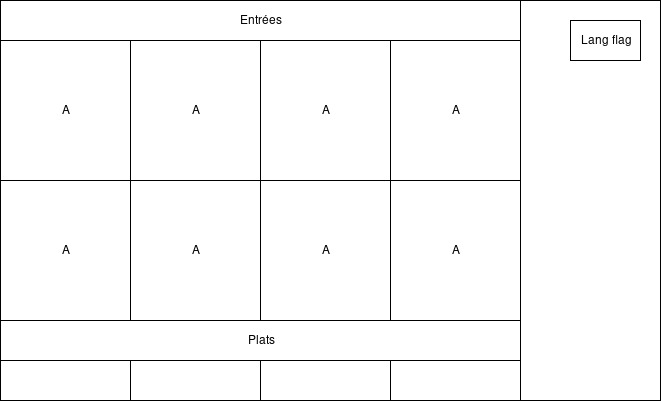
\includegraphics[width=\textwidth]{takeaway_screen.jpg}
\end{center}

\subsubsection{Écran de confirmation}
Après avoir validé la commande, un écran présentant un récapitulatif de la commande invite à confirmer.

\begin{center}
	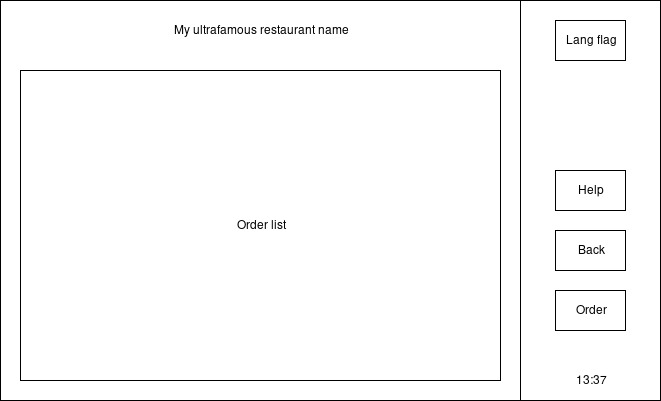
\includegraphics[width=\textwidth]{confirmation_screen.jpg}
\end{center}

\subsubsection{Écran final}

Après la validation de la commande, un écran de remerciement est affiché où l'on donne une estimation du temps
d'attente avant le service. Un champ pour fournir des informations supplémentaires au restaurant est présent.

\begin{center}
	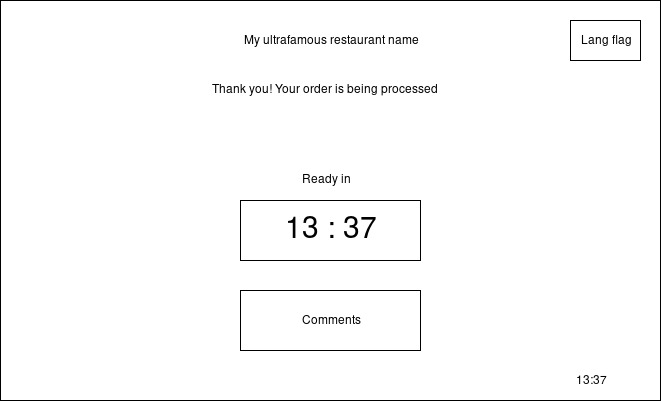
\includegraphics[width=\textwidth]{final_screen.jpg}
\end{center}

\section{Prototype}

\subsection{Informations pratiques}

Le prototype est hébergé sur GitHub à l'adresse suivante : \\
\url{https://github.com/friendshipismagic/pinkie-card.git}.

Ce prototype a été réalisé à l'aide du framework Qt pour plusieurs raisons. Premièrement, nous étions tous familiers
avec cet outil. De plus, comparé à iOS ou Android, c'était le seul qui n'excluait personne dans le groupe pour ne pas
posséder un iPhone ou un téléphone Android.

\subsection{Avancement}

L'avancement du prototype est facile à suive avec l'état du dépôt GitHub. Actuellement, seul l'écran d'introduction
est implémenté.

\end{document}

